\chapter{Leader Election}

In un sistema distribuito, è spesso necessario identificare un nodo che agisce da coordinatore di un determinato task. La presenza di tale entità può essere necessaria per \textit{semplificare} lo svolgimento di un task oppure perché è richiesto per la natura stessa del problema. 

Il problema di scegliere un leader è noto come \textit{leader election} e consiste di scegliere un nodo che agisce da leader da un insieme omogeoneo e simmetrico di individui. Spesso si fa riferimento a questo problema per \textbf{rompere la simmetria} del sistema.

Generalemente, il problema richiede di portare la rete da una configuarazione iniziale in cui tutti i nodi sono in uno stesso stato, diciamo \texttt{asleep}, ad una configurazione finale in cui un nodo è in uno stato \texttt{leader} e tutti gli altri sono in uno stato \texttt{follower}. 

Si può pensare alla leader election come un metodo che \textbf{forza} la restrizione \texttt{unique initiator}, infatti eletto il leader è possibile risolvere il task con protocolli a singolo iniziatore semplicemente ponendo il leader come nodo initiator.

Formalmente, possiamo definire il problema mediente la tripla $\langle P_{init}, P_{final}, R \rangle$

\begin{itemize}
    \item $P_{init}: \forall x \in V: state(x) = \texttt{asleep}$ 
    \item $P_{final}: \exists! x \in V: state(x) = \texttt{leader} \land \forall y \in V \setminus \{x\}: state(y) = \texttt{follower}$ 
    \item $R = \{\texttt{TR, BL, CN}\}$
\end{itemize}

\begin{teorema}[Impossibilità]
    Sotto le restrizioni di $R$, è impossibile risolvere il problema di leader election in modo deterministico.
    \begin{proof}
        La dimostrazione è identica a quella del teorema \autoref{th:MultipleSourcesST}.

        Per avere un idea, consideriamo un sistema con sole due entità $x$ e $y$, inizialmente nello stesso stato \texttt{asleep}. Supponimo l'esistenza di un protocollo $\Pi$, esso deve funzionare sotto qualsiasi condizione e ritardo dei messaggi. Consideriamo per semplicità un sistema sincrono, in cui $x$ e $y$ iniziano la computazione nello stesso istante. Poichè $x$ e $y$ sono indistinguibili, essi eseguiranno le stesse operazioni, invieranno gli stessi messaggi e riceveranno gli stessi messaggi. Di conseguenza, dopo un certo numero di round, $x$ e $y$ saranno ancora nello stesso stato, di conseguenza, se $x$ diventa leader, allora anche $y$ diventa leader, violando la condizione di unicità del leader.
    \end{proof}
\end{teorema}

Questo risultato di \textit{impossibilità} è dato dalla condizione di \textbf{perfetta simmetria} nella rete. Il fenomeno della \textbf{perfetta simmetria} avviene quando una rete ha una struttura totalmente simmetrica, ossia, ogni nodo non è in grado di distiguersi da un altro nodo. Dunque, se tutti i nodi si trovano nello stesso stato interno $\sigma$ ad un instante di tempo $t$, formalmente $\forall x,y \in V: \sigma(x, t) = \sigma(y,t)$, da quel momento in poi si comporteranno in modo identico, dato che avranno la stessa visione del mondo esterno: non potendo comportarsi in maniera diversa, i nodi cambieranno stato allo stesso modo e quindi non è possibile arrivare in una situazione in cui un nodo si definisce \textit{leader} e gli altri nodi \textit{follower}.

È necessario ampliare l'insieme delle restrizioni $R$ per poter risolvere il problema di leader election. Una restrizione banale è quella di \texttt{unique initiator}, che permette di risolvere il problema in modo banale. 

Tuttavia, è possibile risolvere il problema assegnando un identificatore univoco a ciascun nodo e considerare come topologia di rete quella più simmetrica possibile, ovvero un anello.

Sia $G = (V, E)$ un anello con $n$ (non noto) nodi, e sia $id: V \rightarrow \{1, 2, \dots, n\}$ una funzione che assegna un identificatore univoco a ciascun nodo. Ciascun nodo è a conoscenza del proprio identificatore e non conosce gli identificatori degli altri nodi.

\begin{definizione}[Anello]
    Un anello è un grafo $G = (V, E)$ in cui $V = \{x_1, x_2, \dots, x_n\}$ e 
    \[
        E = \{(x_i, x_{i+1}) \in V^2 : 1 \leq i < n\} \cup \{(x_n, x_1)\}.
    \]
    Osserviamo che in un anello, $|E| = |V| = n$. Inoltre, $\forall x \in V, \delta(x) = 2$.
\end{definizione}

\textbf{Osservazione.} Il numero $n$ non è noto ai nodi, per semplicità, possiamo assumere che $id$ sia una permutazione di $\{1, 2, \dots, n\}$, ma non è necessario, basta che sia una funzione iniettiva. Inoltre, assumiamo che ogni nodo condivide una stessa idea di orientamento, ossia i nodi hanno un idea di \textbf{destra} e \textbf{sinistra}.

Sotto queste assunzioni, il problema di leader election si può restringere ad un problema di \textbf{minimum finding (maximum finding)}, ossia trovare il nodo con l'identificatore minimo (massimo) e dichiararlo leader.

\begin{figure}[htbp]
    \centering
    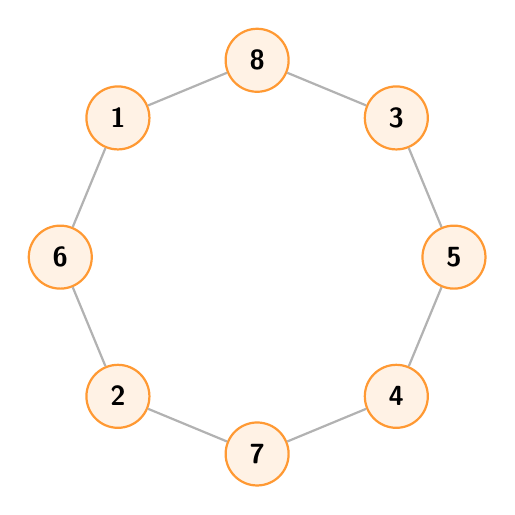
\begin{tikzpicture}[
        mynode/.style={
            circle,
            draw=orange!80,
            fill=orange!10,
            thick,
            minimum size=8mm,
            font=\sffamily\bfseries
        }
    ]
        % Posizionamento nodi con etichette non ordinate
        \foreach \label [count=\i] in {5, 3, 8, 1, 6, 2, 7, 4} {
            \node[mynode] (n\i) at ({(\i-1)*45}:2.5cm) {\label};
        }
    
        % Collegamenti
        \foreach \i [evaluate=\i as \nexti using {int(mod(\i,8)+1)}] in {1,...,8} {
            \draw[thick, gray!60] (n\i) -- (n\nexti);
        }
    \end{tikzpicture}
    
    \caption{Rappresentazione di un anello a 8 nodi.}
    \label{fig:anello_nodi}
\end{figure}

\textbf{Osservazione.} Se consideriamo un albero invece di un anello, basta eseguire la tecnica di saturazione per calcolare il minimo $id(x)$ ed eleggere tale nodo come leader.

\section{All The Way}

Consideriamo il primo protocollo, detto \textbf{all the way}, il quale consiste di far conoscere la propria etichetta a tutti gli altri nodi.

L'idea è la seguente: quando un nodo $x$ si attiva (spontaneamente o dopo aver ricevuto un messaggio), inoltra un messaggio in direzione concorde a tutti (ad esempio a destra) con all'interno $id(x)$. Quando un nodo riceve un messagggio con l'id di qualcun'altro, invia il proprio id se non lo ha ancora fatto, aggiora una variabile locale $min$ che tiene traccia del id minimo ricevuto fin'ora e inoltra il messaggio. 

Possiamo vedere il processo come segue: ogni entità crea un messaggio contenente il proprio id, e questo messaggio attraversa tutta la rete. Ogni entità, per via delle resitrizioni di $TR$, vedrà entro un tempo finito tutti gli id di tutti gli agenti, incluso il valore minimo. Potrà quindi determinare se è il minimo o meno, e quindi, se entrare nello stato \texttt{leader} o \texttt{follower}. 

La domanda che sorge è: quando un nodo capisce di aver visto gli id di tutti gli altri nodi? Il valore $n$ non è noto, perciò è necessario trovare un modo per calcolare il valore $n$.

Il numero $n$ è possibile calcolarlo inserendo un contatore all'interno del messaggio, che viene incrementato ad ogni nodo attraversato. Quando il messaggio torna al nodo di partenza, esso contiene il numero $n$ di nodi presenti nella rete. Dunque, quando un nodo $x$ riceve il suo messaggio da sinitra potrà ricavare il valore $n$ e comportarsi in due modi:
\begin{itemize}
    \item Se $x$ ha ricevuto $n$ messaggi (notiamo che viaggiano $n$ messaggi, ciascuno contenente un id diverso), e $id(x)$ è il minimo, allora $x$ si dichiara \texttt{leader}, altrimenti si dichiara \texttt{follower}.
    \item Se $x$ ha ricevuto $k < n$ messaggi, allora dovrà aspettare di ricevere altri $n - k$ messaggi.
\end{itemize}

In questo modo ogni nodo è in grado di terminare localmente, e solo chi ha l'id minimo si dichiama leader.

Siano
\begin{itemize}
    \item $S = \{\texttt{asleep, awake, follower, leader}\}$
    \item $S_{init} = \{\texttt{asleep}\}$
    \item $S_{final} = \{\texttt{follower, leader}\}$
\end{itemize}

\begin{algorithm}
\caption{All The Way}
\begin{algorithmic}[1]
    \Statex \textbf{Upon} spontaneous awakening:
    \If{state(x) = \texttt{asleep}}
        \State \Call{Initialize}{}
        \State state(x) $\gets$ \texttt{awake}
    \EndIf

    \Statex
    \Statex \textbf{Upon} receiving $msg = \langle \text{"Election"}, id, counter \rangle$ from left:
    \If{state(x) = \texttt{asleep}}
        \State \Call{Initialize}{}
        \State \textbf{send} $\langle \text{"Election"}, id, counter + 1 \rangle$ to right
        \State $\text{min} \gets \min(id, \text{min})$
        \State $\text{count} \gets \text{count} + 1$
        \State state(x) $\gets$ \texttt{awake}
    \EndIf
    
    \Statex
    \If{state(x) = \texttt{awake}}
        \If{$id \neq \text{id}(x)$}
            \State $\text{min} \gets \min(id, \text{min})$
            \State $\text{count} \gets \text{count} + 1$
            \State \textbf{send} $\langle \text{"Election"}, id, counter + 1 \rangle$ to right
            \If{known = \texttt{True}}
                \State \Call{Check}{}
            \EndIf
        \Else
            \State $\text{size} \gets counter$
            \State $\text{known} \gets \texttt{True}$
            \State \Call{Check}{}
        \EndIf
    \EndIf

    \Statex
    \Procedure{Initialize}{}
        \State $\text{count} \gets 1$
        \State $\text{min} \gets \text{id}(x)$
        \State $\text{size} \gets 1$
        \State $\text{known} \gets \texttt{False}$
        \State \textbf{send} $\langle \text{"Election"}, \text{id}(x), 1 \rangle$ to right
    \EndProcedure

    \Statex
    \Procedure{Check}{}
        \If{count = size}
            \If{min = id(x)}
                \State state(x) $\gets$ \texttt{leader}
            \Else
                \State state(x) $\gets$ \texttt{follower}
            \EndIf
        \EndIf
    \EndProcedure
\end{algorithmic}
\end{algorithm}

\subsection{Analisi}

Il protocollo è corretto, in quanto l'assunzione di \texttt{TR} garantisce che ogni nodo prima o poi riceverà le informazioni riguardo le etichette di tutti quanti, dunque riuscirà a calcolare il minimo. Inoltre, la messagge complexity è
\[
    M[\texttt{All The Way}] = O(n^2),
\]
in quanto su ciascun arco passano esattamente $n$ messaggi di $n$ etichette distinte, il numero degli archi è $n$, dunque $n^2$. Possiamo inoltre calcolare la \textbf{bit complexity}, ossia il numero di bit scambiati. Si devono calcolare il numero di bit necessari per rappresentare $id(x)$ e il contatore. Il numero di bit necessari per rappresentare $id(x)$ è $\log_2 id(x)$ (oppure, $\log_2 n$ se consideriamo gli id come na permutazione di $\{1, 2, \ldots, n\}$), mentre il numero di bit necessari per rappresentare il contatore è $\log n$, poichè il contatore può assumere al massimo il valore $n$. Dunque, ogni messaggio contiene $O(\log n)$ bit, e poichè passano $O(n^2)$ messaggi, la bit complexity è
\[
    B[\texttt{All The Way}] = O(n^2 \log n).
\]

Infine, consideriamo l'ideal time complexity. Sia 
\[
    R \cup \{\texttt{Syncronized Clock, Bounded Communication Delay}\}
\]
in questo caso, $T[\texttt{All The Way}] = O(n)$. Il caso peggiore è quando si attiva spontaneamente un solo nodo $x_1$ al tempo $t_0$. Inviando il messaggio al suo vicino $x_2$, esso si attiverà al tempo $t_2$, e cosi via fino al nodo $x_n$ che si attiverà dopo $n-1$ istanti.

\section{As Far}

Questo protocollo è una versione più efficiente di \texttt{All The Way}. Ogni nodo $x$ blocca l'inoltro di tutti gli id che sono maggiori del proprio id, e inoltra solo quelli minori. Allora un messaggio con un certo id viaggia in avanti più a lungo che può.

In questo caso la terminazione locale dei nodi cambia. Infatti,
\begin{itemize}
    \item Sia $l$ il nodo con l'id minimo, allora $l$ prima o poi riceverà un messaggio con il proprio id (il messaggio contenente il suo id sarà l'unico che non verrà mai bloccato), e a quel punto si dichiarerà leader, e invierà un messaggio di notifica in \texttt{broadcast} a tutti gli altri nodi, che si dichiareranno follower e termineranno localmente.
    \item Sia $x$ un nodo con $id(x) > id(l)$, allora $x$ riceverà un messaggio con un id minore del proprio, e quindi inoltrerà il messaggio, ma non riceverà mai un messaggio con il proprio id, dunque non si dichiarerà leader, ma aspetterà di ricevere un messaggio di notifica da parte del nodo leader, e una volta ricevuto, si dichiarerà follower e terminerà localmente.
\end{itemize}

Siano
\begin{itemize}
    \item $S = \{\texttt{asleep, awake, follower, leader}\}$
    \item $S_{init} = \{\texttt{asleep}\}$
    \item $S_{final} = \{\texttt{follower, leader}\}$
\end{itemize}

\begin{algorithm}
\caption{All The Way}
\begin{algorithmic}[1]
    \Statex \textbf{Upon} spontaneous awakening:
    \If{state(x) = \texttt{asleep}}
        \State \Call{Initialize}{}
        \State state(x) $\gets$ \texttt{awake}
    \EndIf

    \Statex
    \Statex \textbf{Upon} receiving $msg = \langle \text{"Election"}, id\rangle$ from left:
    \If{state(x) = \texttt{asleep}}
        \State \Call{Initialize}{}
        \If {$id < min$}
            \State \textbf{send} $\langle \text{"Election"}, id \rangle$ to right
            \State $\text{min} \gets id$
        \EndIf
        \State state(x) $\gets$ \texttt{awake}
    \EndIf
    
    \Statex
    \If{state(x) = \texttt{awake}}
            \If {$id < min$}
                \State \textbf{send} $\langle \text{"Election"}, id \rangle$ to right
                \State $\text{min} \gets id$
            \Else 
                \If {$id = min$}
                    \State state(x) $\gets$ \texttt{leader}
                    \State \textbf{send} $\langle \text{"Leader"}\rangle$ to right
                \EndIf
            \EndIf
    \EndIf

    \Statex
    \Statex \textbf{Upon} receiving $msg = \langle \text{"Leader"}\rangle$ from left:
    \If{state(x) = \texttt{awake}}
        \State state(x) $\gets$ \texttt{follower}
        \State \textbf{send} $\langle \text{"Leader"}\rangle$ to right
    \EndIf

    \Statex
    \Procedure{Initialize}{}
        \State $\text{min} \gets \text{id}(x)$
        \State \textbf{send} $\langle \text{"Election"}, \text{id}(x)\rangle$ to right
    \EndProcedure
\end{algorithmic}
\end{algorithm}

\newpage

\subsection{Analisi}

L'esatto numero di messaggi scambiati dipende dalla disposizione degli id e dal senso di invio. Consideriamo il costo causato dal messaggio \texttt{Election} di un nodo $x$. Tale messaggio viaggerà attraverso l'anello sino a quando non viene ricevuto da un nodo che ha ricevuto in precedenza un $id$ minore, oppure sino a quando non raggiunge il proprio mittente.

Consideriamo il caso peggiore, siano $id_1 < id_2 < \ldots < id_n$ gli id dei nodi nell'anello e supponiamo che l'invio avvenga in senso orario (verso destra). L'$id_1$ attraverserà sempre tutto l'anello avendo quindi un costo di $n$ messaggi, l'$id_2$ attraverserà $n-1$ nodi, venendo bloccato da $id_1$, l'$id_3$ attraverserà $n-2$ nodi, e così via. Dunque, il costo totale è
\[
    M[\texttt{As Far}] = 2n + (n-1) + (n-2) + \ldots + 1 = n + \sum_{i=1}^{n} i = n + \frac{n(n+1)}{2} = O(n^2).
\]

\begin{figure}[htbp]
    \centering
    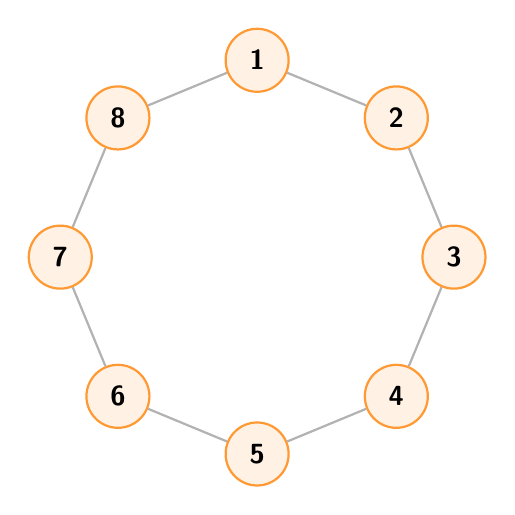
\begin{tikzpicture}[
        mynode/.style={
            circle,
            draw=orange!80,
            fill=orange!10,
            thick,
            minimum size=8mm,
            font=\sffamily\bfseries
        }
    ]
        % Posizionamento nodi in senso ORARIO
        % Usiamo -(\i-1)*45 per invertire la direzione standard di TikZ
        \foreach \i in {1,...,8} {
            \node[mynode] (n\i) at ({90-(\i-1)*45}:2.5cm) {\i};
        }
    
        % Collegamenti (logica invariata, i nodi sono battezzati da n1 a n8)
        \foreach \i [evaluate=\i as \nexti using {int(mod(\i,8)+1)}] in {1,...,8} {
            \draw[thick, gray!60] (n\i) -- (n\nexti);
        }
    \end{tikzpicture}
    
    \caption{Worst case per il protocollo \texttt{As Far}: gli ID sono disposti in ordine crescente in senso orario.}
    \label{fig:worst_case_as_far}
\end{figure}

Il caso migliore si ottiene quando il nodo con etichetta minima inizia il protocollo per primo e la sua etichetta riesce a fare il giro completa della rete prima che le altre vengano inoltrate al proprio vicino. In particolare, il messaggio con etichetta minima viene inoltrato $n$ volte, mentre ogni messaggio con etichetta maggiore viene inoltrato una sola volta, dunque
\[
    M[\texttt{As Far}] = n + (n-1) = O(n).
\]

\newpage

\section{Stage Technique}

Osserviamo che sia nel protocollo \texttt{As Far} che nel protocollo \texttt{All The Way}, le etichette viaggiano lungo l'anello in maniera incontrollata. In particolare, nel protocollo \texttt{As Far} viaggiano finché non vengono filtrati da un nodo con etichetta minore, mentre nel protocollo \texttt{All The Way} viaggiano finché non fanno il giro completo dell'anello. L'idea sarebbe quindi quella di \textbf{controllare} la trasmissione di un'etichetta ad una distanza \textbf{limitata}, e di avere dei \textbf{feedback} per eventualmente bloccare o estendere la trasmissione.

Più precisamente un nodo attivo $x$ eseguo il protocollo in \textbf{stages}, in cui al $i$-esimo stage, $x$ invia la sua etichetta $id(x)$ a destra e sinistra fino a un massimo di distanza di $2^{i-1}$. Così facendo l'etichetta avrà ricoperto un numero di nodi pari a $2^i$, ovvero $2^{i-1}$ a destra e $2^{i-1}$ a sinistra. 

Quando un nodo $y$ riceve l'etichetta di $x$ la inoltrerà sol se $id(y) > id(x)$. Nel caso in cui $y$ inoltrerà $id(x)$ allora vorrà dire che certamente $y$ non sarà mai eletto leader, e quindi passerà in uno stato \texttt{defeated} in cui potrà solamente inoltrare messaggi di altri nodi.

Se l'etichetta $id(x)$ arriva a distanza $2^{i-1}$, allora $x$ ha completato il $i$-esimo stage e verrà rispedita indietro come messaggio di \texttt{feedback}. Quindi se a $x$ arriva la sua etichettà da \textbf{entrambi} i lati, vorrà dire che tutti i nodi a distanza $2^{i-1}$ da lui avranno etichette maggiori, e quindi dovrà inoltrare la richiesta più lontano. In questo caso diciamo che $x$ ha sopravissuto allo stage $i$ e quindi passerà allo stage $i + 1$.

Notiamo che se $x$ non riceve alcun feedback da \textbf{almeno} un lato, allora vorrà dire che esiste un nodo $z$ con $id(z) < id(x)$ entro $2^{i-1}$ passi da $x$, e quindi $x$ non potrà essere eletto leader, dunque passerà in stato \texttt{defeated}.

Infine, quando un nodo $l$ riceverà da destra (o sinistra) il messaggio che aveva inviato a sinistra (o destra), allora $l$ si dichiarerà leader, e invierà un messaggio di notifica in \texttt{broadcast} a tutti gli altri nodi, che si dichiareranno follower e termineranno localmente.

\textbf{Osservazione.} Durante l'esecuzione del protocollo, è possibile che diversi nodi si trovino in diversi stages. Ci si chiede quindi cosa succede se un nodo viene "sconfitto" da un messaggio dello stage $k$ mentre lui si trova nello stage $i < k$. In questo caso, il nodo sconfitto non potrà più essere eletto leader, dunque passerà in stato \texttt{defeated}, e potrà solamente inoltrare messaggi di altri nodi. (NB, il minimo id vince sempre.)

Siano
\begin{itemize}
    \item $S = \{\texttt{asleep, candidate, defeated, follower, leader}\}$
    \item $S_{init} = \{\texttt{asleep}\}$
    \item $S_{final} = \{\texttt{follower, leader}\}$
\end{itemize}

\begin{algorithm}
\caption{Stage Technique}
\begin{algorithmic}[1]
    \Statex \textbf{Upon} spontaneous awakening:
    \If{state(x) = \texttt{asleep}}
        \State \Call{Initialize}{}
        \State state(x) $\gets$ \texttt{candidate}
    \EndIf

    \Statex
    \Statex \textbf{Upon} receiving $msg = \langle \text{"Forth"}, id^*, stage^*, limit^*\rangle$:
    \If{state(x) = \texttt{asleep}}
        \If{$id^* < id(x)$}
            \State \Call{Process-Message}{}
            \State state(x) $\gets$ \texttt{defeated}
        \Else
            \State \Call{Initialize}{}
            \State state(x) $\gets$ \texttt{candidate}
        \EndIf
    \EndIf
    
    \Statex
    \If{state(x) = \texttt{candidate}}
            \If {$id^* < id(x)$}
                \State \Call{Process-Message}{}
                \State state(x) $\gets$ \texttt{defeated}
            \Else 
                \If {$id^* = id(x)$}
                    \State \Call{Notify}{}
                \EndIf
            \EndIf
    \EndIf

    \Statex
    \Statex \textbf{Upon} receiving $msg = \langle \text{"Back"}, id^*\rangle$:
    \If{state(x) = \texttt{candidate}}
        \If{$id^* = id(x)$}
            \State \Call{Check}{}
        \EndIf
    \EndIf

    \Statex
    \Statex \textbf{Upon} receiving $msg = \langle \text{"Notify"}\rangle$:
    \If{state(x) = \texttt{candidate}}
        \State \textbf{send} $\langle \text{"Notify"}\rangle$ to \textbf{other}
        \State state(x) $\gets$ \texttt{follower}
    \EndIf

    \Statex
    \Statex \textbf{Upon} receiving $msg = \langle *\rangle$:
    \If{state(x) = \texttt{defeated}}
        \State \textbf{send} $msg$ to \textbf{other}
        \If {$msg = \langle \text{"Notify"}\rangle$}
            \State state(x) $\gets$ \texttt{follower}
        \EndIf
    \EndIf

    \algstore{stagealgo}
\end{algorithmic}
\end{algorithm}

\newpage

\begin{algorithm}
\caption{Stage Technique}
\begin{algorithmic}[1]
    \algrestore{stagealgo}

    \Statex
    \Procedure{Initialize}{}
        \State $\text{stage} \gets 1$
        \State $\text{limit} \gets dis(stage)$
        \State $\text{count} \gets 0$
        \State \textbf{send} $\langle \text{"Forth"}, \text{id}(x), stage, limit\rangle$ to $N(x)$
    \EndProcedure

    \Statex
    \Procedure{Process-Message}{}
        \State $\text{limit*} \gets \text{limit*} - 1$
        \If {limit* = 0}
            \State \textbf{send} $\langle \text{"Back"}, id^*, stage^*\rangle$ to \textbf{sender}
        \Else
            \State \textbf{send} $\langle \text{"Forth"}, id^*, stage^*, limit^* \rangle$ to \textbf{other}
        \EndIf
    \EndProcedure

    \Statex
    \Procedure{Check}{}
        \State $\text{count} \gets \text{count} + 1$
        \If {count = 2} $\qquad$ //se ho ricevuto sia da destra che da sinistra "Back"
            \State $\text{count} \gets 0$
            \State $\text{stage} \gets \text{stage} + 1$
            \State $\text{limit} \gets dis(stage)$
            \State \textbf{send} $\langle \text{"Forth"}, id(x), stage, limit\rangle$ to $N(x)$
        \EndIf
    \EndProcedure

    \Statex
    \Procedure{Notify}{}
        \State \textbf{send} $\langle \text{"Notify"}\rangle$ to \textbf{right}
        \State state(x) $\gets$ \texttt{leader}
    \EndProcedure
\end{algorithmic}
\end{algorithm}

\subsection{Analisi}

La correttezza del protocollo deriva dalla sua definizione. Infatti, solamente l'etichetta minima sarà in grado di sopravvivere a tutti gli stages (e quindi a fare un giro completo), e quindi di dichiararsi leader, mentre tutte le altre etichette saranno bloccate da un nodo con etichetta minore, e quindi si dichiareranno follower.

Analizziamo ora la message complexity del protocollo. Considerando che il ritardo dei messaggi è \textbf{impredicibile} si osserverà che ad un tempo $t$ non solo ci saranno nodi in stati differenti, ma anche che ci saranno nodi \textit{candidati} in \textbf{stages differenti}. Infatti, non essendoci una \texttt{Message Ordering}, può capitare che dei messaggi sorpassino degli altri. Perciò, faremo un'analisi procedendo per \textbf{logical stages}, ossia, al $i$-esimo stage, considereremo solamente i messaggi relativi allo stage $i$, e faremo un'analisi indipendente per ogni stage (non consideriamo che differenti nodi possono eseguire uno stesso stage in tempi differenti, come abbiamo visto, se un nodo nello stage $i-1$ riceve un messaggio da un nodo nello stage $i$, vince sempre il nodo con l'etichetta minore (approccio greedy)).

\begin{teorema}[Message Complexity]
    La message complexity del protocollo \texttt{Stage Technique} è
    \[
        M[\texttt{Stage Technique}] = O(n \log n).
    \]
    \begin{proof}
        Sia $i > 1$, definiamo $n_i$ il numero di nodi che iniziano lo stage $i$, ovvero quelli sopravissuti allo stage $i-1$. Osserviamo che 
        \[
            n_i \leq \frac{n}{2^{i-2} + 1}, 
        \]
        in quanto, se un nodo sopravvive allo stage $i-1$, allora tutti i nodi entro una distanza di $2^{i-2}$ da lui hanno etichetta maggiore, dunque, in totale, ci sono al massimo $\frac{n}{2^{i-2}}$ nodi che possono sopravvivere allo stage $i$ (un solo nodo su $2^{i-2}$ può sopravvivere).
        \begin{figure}[htbp]
            \centering
            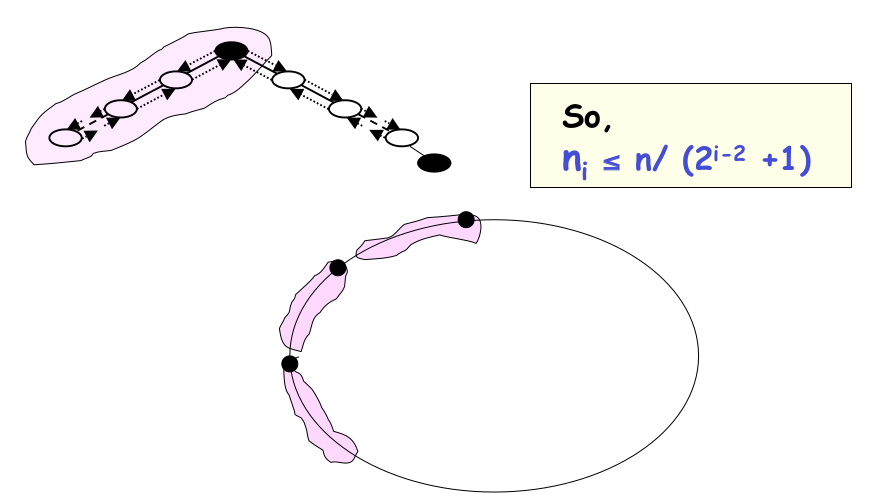
\includegraphics[width=0.8\textwidth]{images/stage_tecnique_msg.png}
            \caption{Nodi che sopravvivono allo stage $i$.
            \label{fig:stage_tecnique_msg}}
        \end{figure}
        
        Non ci può essere più di un sopravvissuto ogni $2^{i-2}$ nodi in quanto se ce ne fossero di più, per esempio $x$ e $y$, vorrebbe dire che $x$ ed $y$ si sono scambiati le etichette senza però che uno dei due venisse "sconfitto", e ciò implicherebbe che $id(x) < id(y) < id(x)$.

        Contiamo ora il numero di messaggi scambiati durante lo stage $i$. Abbiamo due tipologie di messaggi, quelli di tipo \texttt{Forth} e quelli di tipo \texttt{Back}. 
        \begin{description}
            \item[FORTH:] Ogni nodo candidato $x$ inoltra la sua etichetta ad \textbf{al più} $2 \cdot 2^{i-1} = 2^i$ nodi, per un totale di $n_i \cdot 2^i$
            \item[BACK:] Poiché nella fase $i$ sopravviveranno $n_{i+1}$ candidati, per ognuno verranno necessariamente trasmessi altri $2 \cdot 2^{i-1} = 2^i$ messaggi di feedback, per un totale di $n_{i+1} \cdot 2^i$.
        \end{description}
        Infine, rimangono i nodi \texttt{defeated}, che sono $n_i - n_{i+1}$. Questi riceveranno al massimo un messaggio di tipo \texttt{Back}, per un massimo di $2^{i-1}$ ulteriori messaggi, dunque, in totale, \textbf{al più} $2^{i-1} \cdot (n_i - n_{i+1})$ messaggi.
        
        Perciò, complessivamente, nella fase $i > 1$,
        \begin{align*}
            M[\texttt{stage}_i] 
            &= 2n_i2^{i_1} + 2n_{i+1}2^{i-1} + (n_i - n_{i+1})2^{i-1} = (3n_i + n_{i+1})2^{i-1} \\
            &\leq \left( 3 \bigg\lfloor \frac{n}{2^{i-2} + 1} \bigg\rfloor + \bigg\lfloor \frac{n}{2^{i-2} + 1} \bigg\rfloor \right)2^{i-1} \\
            &< \left( 3  \frac{n}{2^{i-2} + 1} + \frac{n}{2^{i-2} + 1} \right)2^{i-1} \\
            &< \left( 4  \frac{n}{2^{i-2}} \right)2^{i-1} \\
            &= 6n + n = 7n.
        \end{align*}
        
        \textbf{Osservazione.} Il numero di messaggi scambiati durante lo stage $1$ è diverso, poichè il caso peggiore si ha quando tutti i nodi sono iniziatori. In questo caso 
        \[
            n_2 \leq \frac{n}{2^0 + 1} = \frac{n}{2}
        \]
        I nodi che sopravvivono allo stage $1$ pagano individualmente 2 per \texttt{Forth} e 2 per \texttt{Back}, mentre i nodi che vengono sconfitti pagano individualmente 2 per \texttt{Forth} 1 per \texttt{Back}, in totale,
        \[
            M[\texttt{stage}_1] = 4n_2 + 3n - 3n - 3n_2 = n_2 + 3n < 4n.
        \]

        \textbf{Numero di stage.} Rimane solo da dimostrare che il numero di stage è $O(\log n)$. Sia $i^*$ lo stage in cui un nodo si dichiara leader, ossia quando riceverà da un lato il messaggio che ha inviato dal lato opposto, allora
        \[
            i^* = \min \{i \in \mathbb{N} : 2^{i-1} \geq n\} \iff i^* = O(\log n)
        \]
        Dunque il numero necessari di stage è $O(\log n)$, e poiché in ogni stage vengono scambiati al più $7n$ messaggi, la message complexity totale è
        \[
            M[\texttt{Stage Technique}] = \sum_{i=1}^{\log n} M[\texttt{stage}_i] + M[\texttt{stage}_1] = O(n \log n).
        \]
    \end{proof}
\end{teorema}

\newpage

\section{Mesh Architecture}
\begin{definizione}[Mesh]
    Una mesh è un grafo $\mathcal{M} = (V, E)$ dove:
    \begin{align*}
        V &= \{x_{i,j} : 1 \leq i \leq a,\ 1 \leq j \leq b\}, \quad |V| = n = ab \\
        E &= \{(x_{i,j}, x_{i+1,j}) : 1 \leq i < a, 1 \leq j \leq b\} \\
          &\quad \cup \{(x_{i,j}, x_{i,j+1}) : 1 \leq i \leq a, 1 \leq j < b\}, \quad |E| = m = 2ab - a - b.
    \end{align*}
    Una mesh è una griglia rettangolare di dimensioni $a \times b$ dove ogni nodo è collegato ai suoi vicini orizzontali e verticali.
\end{definizione}

\begin{figure}[htbp]
    \centering
    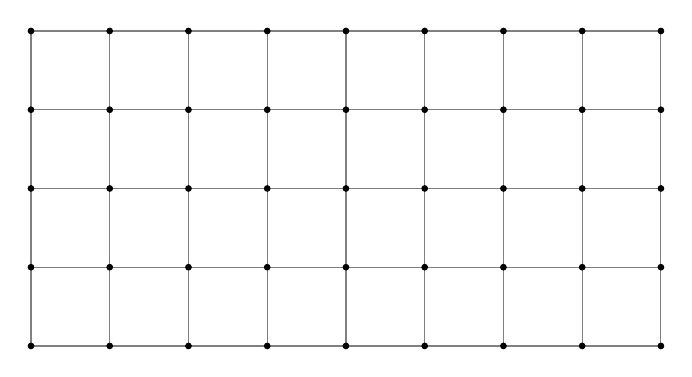
\begin{tikzpicture}
        \draw[thin, gray] (0,0) grid (8,4);

        \foreach \x in {0,...,8}
            \foreach \y in {0,...,4}
            {
                \filldraw[black] (\x,\y) circle (1pt);
            }
    \end{tikzpicture}
    \caption{Rappresentazione di una mesh $9 \times 5$.}
    \label{fig:mesh_9x5}
\end{figure}

In una mesh, possiamo distiguirere tre tipi di nodi (è una topologia \textbf{asimmetrica}):
\begin{itemize}
    \item \textbf{Corner nodes}: sono i nodi che si trovano agli angoli della griglia, e hanno grado 2.
    \item \textbf{Edge nodes}: sono i nodi che si trovano sui bordi della griglia, ma non agli angoli, e hanno grado 3 e ve ne sono $2(a+b)-4$.
    \item \textbf{Inner nodes}: sono i nodi che si trovano all'interno della griglia, e hanno grado 4 e ve ne sono $(a-2)(b-2)$.
\end{itemize}

\subsection{Protocollo}

Consideriamo il sottografo indotto dai nodi \textbf{corner} e dai nodi \textbf{edge}, che formano un anello. Eseguiamo su tale anello un protocollo di leader election per eleggere un leader tra i nodi \textbf{corner}. Essi saranno gli unici candidati, mentre i nodi \textbf{edge} avranno solo il ruolo di inoltro. Una volta eletto il leader, esso esegue una \texttt{broadcast} a tutta la rete, e ogni nodo si dichiara follower e termina localmente.

Il protocollo consiste di tre fasi:
\begin{enumerate}
    \item \textbf{Wake Up:} Ogni initiator ($k$) invia un messaggio di \texttt{wake-up} a tutti i suoi vicini. Ogni nodo non iniator che riceve il messagio di \texttt{wake-up}, lo invia agli altri vicini, in totale si scambiano
    \[
        M[\texttt{Wake Up}] = 3n + k = O(n).
    \]
    \item \textbf{Election on the Ring: } Poichè i nodi sanno di essere o edge o corner, possono eseguire un protocollo di leader election sull'anello formato da questi nodi. I nodi corner sono gli unici candidati, che inviano i propri id, mentre i nodi edge si limitano ad inoltrare i messaggi. Quindi, un nodo sa che ci sono esattamente 4 candidati, e una volta che ha ricevuto 4 id diversi può calcolare il minimo e dichiararsi o leader o follower e terminare localmente. La message complecity è:
    \[
        M[\texttt{Election on the Ring}] = O(a + b) = O(\sqrt{n}),
    \]
    poichè su ogni link dell'anello passano al più 4 messaggi, e l'anello è formato da $2(a+b)-4$ nodi.
    \item \textbf{Broadcast: } Il nodo leader esegue una \texttt{broadcast} a tutta la rete, e ogni nodo si dichiara follower e termina localmente. La message complexity è
    \[
        M[\texttt{Broadcast}] = O(n),
    \]
\end{enumerate}

\section{Randomized Algorithm}

Abbiamo visto che il problema della leader election non è risolvibile in modo deterministico in una rete in cui i nodi sono anonimi, ossia non esiste uno etichettamento univoco dei nodi. 

Consideriamo ora una anello $G = (V, E)$ di dimensione $n$, dove i nodi sono \textbf{anonimi}, e conoscono la topologia della rete e il numero di nodi $n$. In questo caso, è possibile risolvere il problema della leader election in modo \textbf{randomizzato}.

Ciascun nodo $x \in V$ sceglie, indipendentemente dagli altri nodi, la sua etichetta 
\[
    id(x) \xleftarrow{u.a.r.} [m] = \{1, \dots, m\},
\]
dove $m$ è un parametro che dipende da $n$ e che verrà scelto in modo opportuno, sperando che non esistano due nodi con la stessa etichetta. A questo punto, i nodi eseguono uno dei protocolli visti in precedenza (\texttt{All The Way, As Far, Stage Technique}) per eleggere un leader tra i nodi che hanno scelto l'etichetta minima.

Formalemente, il protocollo $\mathcal{RL}(G, n; m)$ è il seguente ($m$ è un parametro che dipende da $n$ e che verrà scelto in modo opportuno):
\begin{enumerate}
    \item \textbf{Wake-up:} Viene eseguito un protocollo di wake-up, in modo che tutti i nodi si attivino.
    \item \textbf{Random ID Generation:} Ogni nodo $x$ sceglie, indipendentemente dagli altri nodi, la sua etichetta $id(x)$ in modo uniforme a caso da $[m]$.
    \[
        id(x) \xleftarrow{u.a.r.} [m] = \{1, \dots, m\},
    \]
    \item \textbf{Leader Election:} I nodi eseguono uno dei protocolli \textit{deterministici} di leader election visti in precedenza, per eleggere un leader tra i nodi che hanno scelto l'etichetta minima.
\end{enumerate}

\subsection{Analisi}

Analizziamo ora la corretteza del protocollo, la message complexity ovviamente dipende da quale protocollo deterministico viene scelto, che abbiamo già analizzato, dunque ci concentriamo sulla probabilità di successo del protocollo.

Dobbiamo fare un'analisi probabilistica del protocollo. Innanzitutto definiamo lo spazio di probabilità, che è dato da tutte le possibili assegnazioni di etichette ai nodi, dunque
\[
    \Omega = [m]^n = \{(id(x_1), id(x_2), \ldots, id(x_n)) : id(x_i) \in [m],\ 1 \leq i \leq n\}.
\]

Osserviamo che un \textbf{evento sufficiente} (ma \textbf{non necessario}) affiché il protocollo termini \textbf{correttamente} è:

\[
    \mathcal{B} = "\text{non esistono due nodi differenti } u, w \in V,\ u \neq w:\ id(u) = id(w)"
\]

L'evento $\mathcal{B}$ è sufficiente perché se non esistono due nodi con la stessa etichetta, allora esiste un nodo con etichetta minima, e tale nodo sarà l'unico candidato, dunque verrà eletto leader, e tutti gli altri nodi si dichiareranno follower e termineranno localmente. Tuttavia, $\mathcal{B}$ non è necessario perché è possibile che esistano due nodi $u, v \in V$ con $u \neq v$ e $id(u) = id(v)$ ma che esista un nodo $w$ con $id(w) < id(u) = id(v)$, e quindi $w$ sarà l'unico candidato, e verrà eletto leader, e tutti gli altri nodi si dichiareranno follower e termineranno localmente.

Osserviamo che possiamo modellare il problema come un problema di \textbf{urne e palline} (\textit{Balls-into-Bins Process}), in cui abbiamo $n$ palline (i nodi) e $m$ urne (le possibili etichette), e ogni pallina viene lanciata in modo uniforme a caso in una delle $m$ urne. L'evento $\mathcal{B}$ si verifica se e solo se tutte le palline finiscono in urne diverse, ossia non esistono due palline che finiscono nella stessa urna.

Calcoliamo ora la probabilità che si verifichi l'evento $\mathcal{B}$. 
\[
    \mathcal{P}(\mathcal{B}) = 1 - \mathcal{P}(\overline{\mathcal{B}}) = 1 - \mathcal{P}("\text{esistono due nodi } u, w \in V,\ u \neq w:\ id(u) = id(w)")
\]

Per ogni $i \in [m]$, definiamo l'evento 
\[
    \overline{\mathcal{B}}_{i} = "\text{esistono due nodi } u, w \in V,\ u \neq w:\ id(u) = id(w) = i".
\]

Possiamo vedere l'evento $\overline{\mathcal{B}_i}$ come "almeno due palline finiscono nell'urna $i$", quindi,

Tale evento può essere modellato come l'unione di v.a. binamiali.

\begin{align*}
    \mathcal{P}(\overline{\mathcal{B}_i}) 
    &= \mathcal{P} \left( \bigcup_{k=2}^{n} \{ \text{esistono } k \text{ palline nell'urna } i \} \right) \\
    \text{unione di eventi disgiunti } &= \sum_{k=2}^{n} \mathcal{P} (\text{esistono } k \text{ palline nell'urna } i) \\
    &= \sum_{k=2}^{n} \binom{n}{k} \left( \frac{1}{m} \right)^k \left( 1 - \frac{1}{m} \right)^{n-k} \leq \sum_{k=2}^{n} \binom{n}{k} \left( \frac{1}{m} \right)^k \\
    \text{Stirling's approx } &\leq \sum_{k=2}^{n} \left( \frac{ne}{k} \cdot \frac{1}{m}\right)^k \leq O\left(\frac{n^2}{m^2}\right) + \sum_{k=3}^{n} \left( \frac{ne}{k} \cdot \frac{1}{m}\right)^k \\
    &\leq O\left(\frac{n^2}{m^2} + \frac{n^4}{m^3}\right)
\end{align*}

Adesso, possiamo calcolare la probabilità che si verifichi l'evento $\overline{\mathcal{B}}$, ossia che esistano due nodi con la stessa etichetta, utilizzando l'unione di eventi:
\begin{align*}
    \mathcal{P}(\overline{\mathcal{B}})
    &= \mathcal{P} \left( \bigcup_{i=1}^{m} \overline{\mathcal{B}_i} \right) \\
    \text{union bound } &\leq \sum_{i=1}^{m} \mathcal{P}(\overline{\mathcal{B}_i}) \\
    &\leq m \cdot O\left(\frac{n^2}{m^2} + \frac{n^4}{m^3}\right) = O\left(\frac{n^2}{m} + \frac{n^4}{m^2}\right)
\end{align*}

Ponendo ora $m = n^3$, avremo che tale probabilità sarà al più
\[
    \mathcal{P}(\overline{\mathcal{B}}) = O\left(\frac{n^2}{n^3} + \frac{n^4}{n^6}\right) \in O\left(\frac{1}{n}\right).
\]

Possiamo quindi concludere che per $m \geq n^3$, l'esecuzione del protocollo $\mathcal{RL}(G, n; m)$ porterà la rete in una configurazione finale accettabile con \textbf{alta probabilità (w.h.p.)} 
\[
    \mathcal{P}(\mathcal{B}) = 1 - O\left(\frac{1}{n}\right)
\]
